\documentclass{article}

\usepackage{pdfcomment}
\usepackage[margin=1in]{geometry}
\usepackage{xcolor}
\usepackage{graphicx}

\newcommand{\note}[2]{\pdfmargincomment[color=yellow,author=#1,open=true]{#2}}
\newcommand{\todo}[1]{\color{red}\textbf{TODO:}#1\color{black}}

\title{Numerical error propagation in the HCP structural pre-processing pipelines}

\author{M. Ali Salari, Lalet Scaria, Gregory Kiar, Lindsay B. Lewis,
  Alan C. Evans, Tristan Glatard}

\begin{document}

\maketitle

\abstract{This paper is a reproducibility study of the work in~\cite{glasser2015multi}.}

\section{Introduction}

Operating systems are known to have an effect on the results produced
by neuroimaging pipelines~\cite{Gronenschild2012, Glatard2015},
presumably due to the creation, propagation and amplification of small
numerical errors across the pipelines.  Such errors highlight
numerical instability which is also likely to appear as a result of
other types of small perturbations such as acquisition and parametric
noise. However, the precise causes of
such instabilities and the path along which they propagate in the
pipelines are unclear.  We present a technique to identify the
processes in a pipeline that create numerical errors along the
execution, and we apply this technique to the HCP structural
pre-processing pipelines.


Groenschild \emph{et al.} first identified the effect of operating
systems on Freesurfer
results~\cite{Gronenschild2012}. In~\cite{10.3389/fninf.2015.00012} we
quantified this effect on some of the main neuroimaging pipelines
including several FSL pipelines, CIVET and Freesurfer. In this work we
aim at evaluating this effect on the work in~\cite{glasser2015multi}.
\todo{Link this to Lindsay's HBM 2017 poster and to Redolfi et al.}

The operating system is defined here as a consistent set of software
packages organized in a trusted repository.

The operating system is not the only part of the computational
environment that may hamper reproducibility. The work
in~\cite{diethelm2012limits} mentions reproducibility issues coming
from parallelization.

Notes:
\begin{itemize}
  \item Reproducibility has several other aspects, see, e.g.,
\url{https://medium.com/@lorenaabarba/barba-group-reproducibility-syllabus-e3757ee635cf#.ty3zmgd4k}
 \item James P Turner, speaker in INCF 2016 Track B, is looking at numerical stability on GPUs. And reproducibility.
 \item For an overview of variability accross analysis methods in fMRI, see \url{http://journal.frontiersin.org/article/10.3389/fnins.2012.00149/full}.
 \item For a general overview in fMRI, see \url{http://www.nature.com/nrn/journal/vaop/ncurrent/box/nrn.2016.167_BX3.html}
\end{itemize}
   
\section{Materials and Methods}

\subsection{Data and Processing}

We randomly selected 6 subjects from the HCP data release S500 and
processed them with the HCP structural pre-processing pipelines
v3.19.0 (PreFreeSurfer and FreeSurfer)~\cite{Glasser2013} in CentOS
6.8 and CentOS 7.2 using Docker containers. We collected the
provenance trace (tree of executed processes and files accessed in
read or write mode) for one subject using system-call interception as
provided by the reprozip tool~\cite{5}.

Notes:
\begin{itemize}
\item Point to the Docker images
\end{itemize}

\paragraph{Pipelines}

Described in~\cite{glasser2013minimal}.

\paragraph{Processing environment}

See Lalet's thesis. Boutiques, CBRAIN, wrappers scripts, etc.

The pipeline was launched twice in the same
environment to detect any use of pseudo-random numbers. We
made sure that the results produced by these two executions were
identical.

\begin{itemize}
  \item monitor.sh - For monitoring the hardware details and software library versions
  \item create-execution.sh for keeping the input directories unmodified and thus preventing modification of input files.
  \item checksums.sh - To make sure that the files are not corrupted while transferring or processing the subjects.
  \item command-line-script.sh - For submitting the PreFreeSurfer Pipeline script with the right paramets.
  \item command-line-script.sh - For submitting the PreFreeSurfer Pipeline script with the right paramets.
  \item Checksums to detect file corruption.
  \item Hardware information is captured to make sure that differences are not coming from, e.g., different CPUs (when on cluster).
  \item Checksum of Docker container is recorded to make sure that the same container was used all over. Also, list of packages with versions is printed for every task. 
  \item Multiple runs are executed per condition to detect potential intra-condition differences (e.g., use of pseudo-random numbers).
\end{itemize}

\subsection{Measuring differences}

 We computed a file difference matrix between files produced in each
 operating system based on file checksums as in~\cite{Scaria2017}.

Binary and non-binary.

See Lalet's thesis

Describe the scripts that will be written to compare results.

Describe how metrics (distances?) are associated to file types (based
on regexp) and used to compute distance matrices. Including metrics to
implement the safeguards. Report comparison algorithm (see Google
Drive).


\subsection{Pipeline analysis: Characterizing differences}

From the reprozip trace and file error matrix, we classified
 processes depending whether they created errors, removed errors, or
 did not have any impact. To control the propagation of errors in the
 pipeline and allow for the classification of all processes, process
 classification was done in an iterative manner in which we
 artificially corrected errors by replacing the original process by a
 file copy from the results obtained in the other operating system. In
 this way, we were able to pinpoint the origin of the errors measured
 in the pipeline.

 Once differences between conditions are quantified, we automatically identify the steps in the pipeline responsible for such differences as follows:
\begin{itemize}
\item Capture the execution trace using reprozip (based on system-call interception).
\item Query the reprozip trace to retrieve the executable(s) that wrote in a given file.
\end{itemize}

\section{Results}

Show lists of packages used with version. Focus on important
differences (e.g.: python interpreter, gcc if relevant) and explain
why these packages are important.

Show results of the comparison.

\subsection{Inter-OS differences}


\paragraph{Binary differences}


Among the 117 data files produced by PreFreeSurfer, 23 did not have any error for any subject, 92 had errors 
for all subjects and 2 had errors for 1 subject only. 

In a previous study~\cite{Scaria2017}, we showed that
pre-processing pipelines of the Human Connectome
Project~\cite{Glasser2013} were sensitive to operating system
variation (see Figure \ref{fig:1}).
\begin{figure}
%  \includegraphics{brain\_classification}
  \caption{Tissue classification produced by the HCP pre-processing
    pipelines on subject 105216 (CentOS 6 vs CentOS 7). \todo{Represent this in a different way.}}
  \label{fig:1}
\end{figure}

\subsection{Pipeline analysis}

Figure \ref{fig:2} shows the annotated provenance graph of the
PreFreeSurfer pipeline executed on CentOS6 and CentOS7.  Processes
that created errors are shown in red, processes that removed errors
are in blue, and other processes are in green.  Squares denote
processes for which the classification is uncertain, due to temporary
files that were removed during the execution. Black edges link
sub-processes to their parents while dashed edges denote file
dependencies between processes (green edges: files with no errors; red
edges: files with errors; yellow edges: temporary files).  The
processes that introduce errors in PreFreeSurfer are: linear
registration with “\emph{FLIRT}” (8 occurrences, in ACPC Alignment,
BrainExtraction, DistortionCorrection, AtlasRegistration), non-linear
registration with “\emph{FNIRT}” (3 occurrences, in BrainExtraction
and AltasRegistration), image warping with “\emph{new\_invwarp}” (3
occurrences, in BrainExtraction and AtlasRegistration).  In addition,
errors were observed in image mean and standard-deviation computations
with “\emph{fslstats}” (3 occurrences in BiasFieldCorrection), and in
masked image extrapolation with “\emph{fslmaths}” (1 occurrence, in
BiasFieldCorrection).  Besides, transformation format conversion with
“\emph{convertwarp}” (2 occurrences, in DistortionCorrection) was able
to remove errors.

\todo{Check if a given file is written by only one process (add a safeguard in your code).}

\begin{figure}
  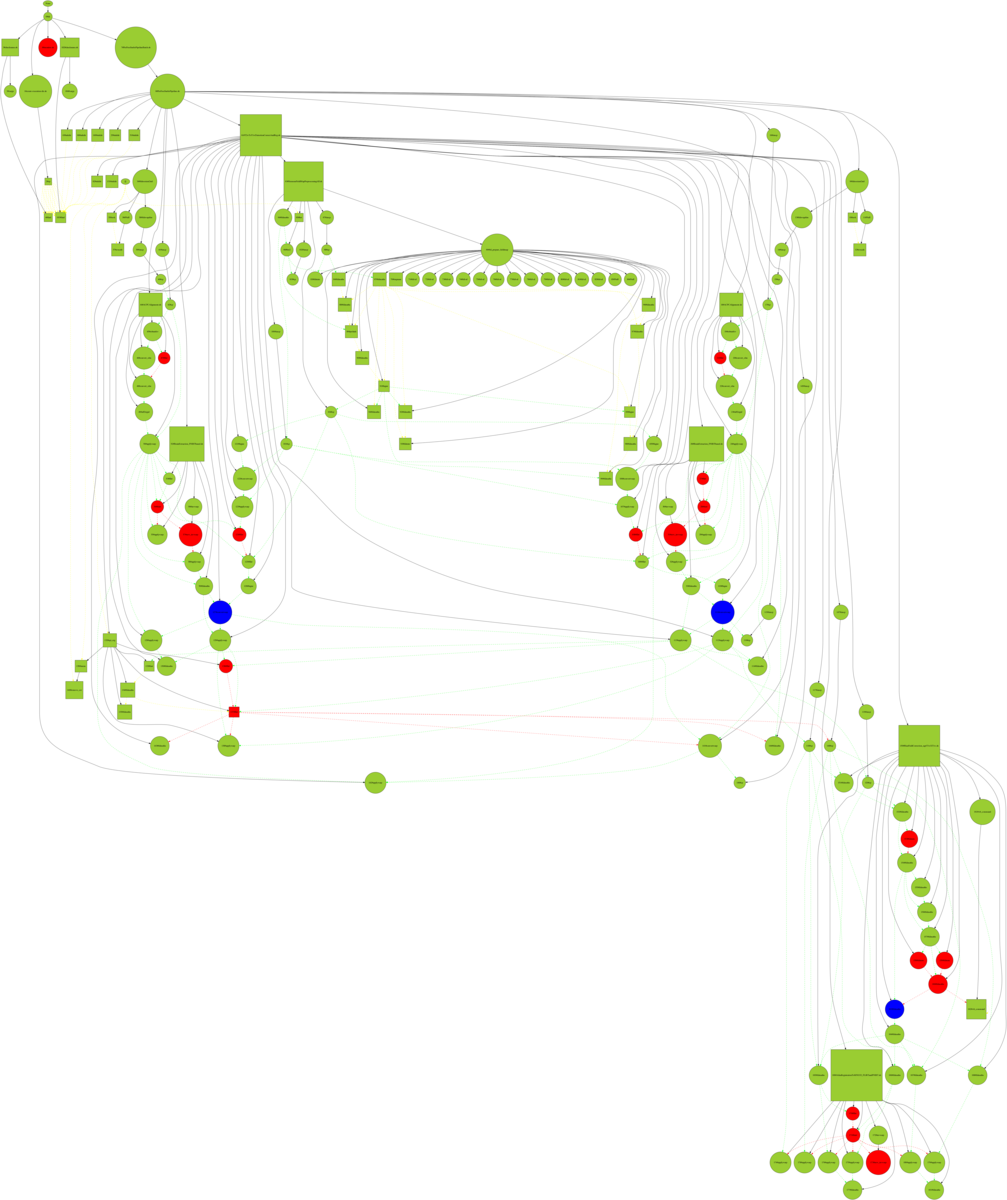
\includegraphics[width=\linewidth]{images/graph}
  \caption{An annotated provenance graph from the PreFreesurfer pipeline. Processes that created errors are in red. 
Full-resolution image available at \url{https://drive.google.com/open?id=174yyn8SuVOUcK5aRVw0bagjDanLD0FLt}.}
  \label{fig:2}
\end{figure}

\section{Discussion}

Discuss the results.

Mention that this was only possible because the unprocessed data was shared in the first place.

DICOM to Nifti conversion was out of scope and may introduce other issues.

\section{Conclusion}

Conclude and highlight future work.

The numerical instability in the PreFreesurfer HCP pipeline arises mainly from linear and non-linear registration processes 
implemented in FSL FLIRT and FNIRT. These processes need to be reviewed to understand and correct the cause of instabilities. 
In this correction process, accuracy has to be considered in addition to stability. Our technique is able to 
characterize the stability of a pipeline’s components automatically, but it also suffers from limitations as it cannot deal with: 
(1) results that are not written to disk (values processed in memory); (2) temporary files (3) files that are written by more than one process.


\section{Acknowledgments}

CBRAIN team. Compute Canada(Calcul Quebec).

\bibliographystyle{plain}
\bibliography{biblio}

\end{document}
